\documentclass{../notes}

\title{商务智能 HW04}

\begin{document}
    \maketitle

    展开后的RNN结构如图\ref{fig:rnn-structure}所示:

    \begin{figure}[ht]
        \centering
        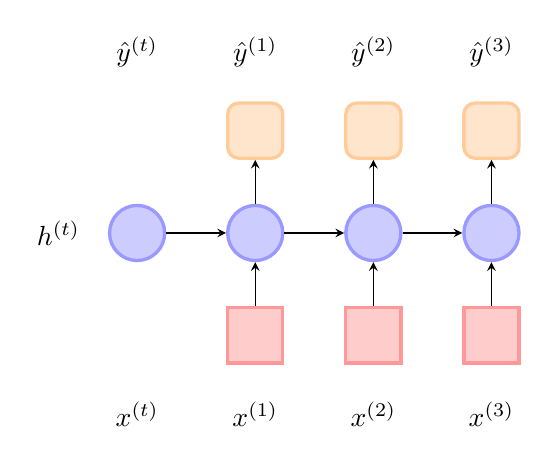
\begin{tikzpicture}
            [
                InputNode/.style={rectangle, draw=red!40, fill=red!20, very thick, minimum size = 7mm},
                HiddenNode/.style={circle, draw=blue!40, fill=blue!20, very thick, minimum size = 7mm},
                OutputNode/.style={rectangle, rounded corners, draw=orange!40, fill=orange!20, very thick, minimum size = 7mm},
                Connection/.style={-stealth}
            ]
            \node (Hidden_00){};
            \node [below of=Hidden_00]{$\bs x^{(t)}$};
            \foreach \t [evaluate=\t as \p using int(\t-1)] in {1, 2, 3} {
                \node[InputNode, right of=Hidden_0\p, xshift=0.5cm] (Hidden_0\t){};
                \node[below of=Hidden_0\t]{$\bs x^{(\t)}$};
            }
            \foreach \t in {0, 1, 2, 3} {
                \node[HiddenNode, above of=Hidden_0\t, yshift=0.3cm] (Hidden_1\t) {};
            }
            \foreach \t [evaluate=\t as \n using int(\t+1)] in {0, 1, 2} {
                \draw[Connection] (Hidden_1\t) -> (Hidden_1\n);
            }
            \node [left of=Hidden_10]{$\bs h^{(t)}$};

            \node [above of=Hidden_10, yshift=0.3cm](Hidden_20){};
            \node [above of=Hidden_20]{$\hat {\bs y}^{(t)}$};
            \foreach \t in {1, 2, 3} {
                \node[OutputNode, above of=Hidden_1\t, yshift=0.3cm] (Hidden_2\t){};
                \node[above of=Hidden_2\t]{$\hat {\bs y}^{(\t)}$};
                \foreach \l [evaluate=\l as \n using int(\l + 1)] in {0, 1} {
                    \draw[Connection] (Hidden_\l\t) -> (Hidden_\n\t);
                }
            }
        \end{tikzpicture}
        \caption{展开后的RNN结构}
        \label{fig:rnn-structure}
    \end{figure}

    不考虑输入批次,令$\bs x^{(i)}$为列向量。设隐藏层的输入权重、循环权重,输出权重分别为$\bs W_i, \bs W_h, \bs W_o$,输入偏置、循环偏置、输出偏置分别为$\bs b_i, \bs b_h, \bs b_o$,令$\bs b = \bs b_i + \bs b_h$。激活函数为$f(\cdot) = \tanh$。对于$t$时刻,计算过程如下所示:

    \begin{enumerate}[label=\textit{第\arabic*步}]
        \item 计算中间变量$\bs \alpha^{(t)} = \bs W_i\bs x^{(t)} + \bs W_h\bs h^{(t-1)} + \bs b$(需要在反向传播过程中使用)
        \item 计算隐藏层输出$\bs h^{(t)} = f\left(\bs \alpha^{(t)}\right)$
        \item 计算中间变量$\bs \beta^{(t)} = \bs W_o \bs h^{(t)} + \bs b_o$
        \item 计算输出层输出$\hat {\bs y}^{(t)} = f\left(\bs \beta^{(t)}\right)$
    \end{enumerate}

    设交叉熵函数为$g(\cdot)$,进行一次训练的损失函数为$G = \sum_{t} g\left(\hat {\bs y}^{(t)}, \bs y^{(t)}\right)$,$t$时刻$g$对$\hat {\bs{y}}^{(t)}$的偏导数为$g'^{(t)} = \partial g/ \partial \hat {\bs{y}}^{(t)}$。定义$\nabla^{(t)}$为对输出$\hat {\bs y}$进行反向传播的的梯度增量,即$\nabla (\cdot) = \sum_t \nabla^{(t)} (\cdot)$。定义全1矩阵$\bs 1_{X}$为形如$\bs X$的矩阵,且其中所有元素均为1。反向传播过程如下:

    \begin{enumerate}[label=\textit{第\arabic*步}]
        \item 对于$t$时刻,计算$\bs b_o$的偏导数为$\nabla^{(t)} \bs b_o = g'^{(t)}f'\left(\bs \beta^{(t)}\right)\bs 1_{\bs h^{(t)}}$。
        \item 对于$t$时刻,计算$\bs W_o$的偏导数为$\nabla^{(t)} \bs W_o = g'^{(t)}f'\left(\bs \beta^{(t)}\right)\bs h^{(t)}$
        \item 对于$t$时刻,计算$\bs b_h, \bs b_i$的偏导数为$\nabla^{(t)} \bs b_h = \nabla^{(t)} \bs b_i = g'^{(t)}f'\left(\bs \beta^{(t)}\right)\bs h^{(t)} f'\left(\bs \alpha^{(t)}\right)\bs 1_{\bs h^{(t-1)}}$
        \item 对于$t$时刻,计算$\bs W_h$的偏导数为$\nabla^{(t)} \bs W_h = g'^{(t)}f'\left(\bs \beta^{(t)}\right)\bs h^{(t)}f'\left(\bs \alpha^{(t)}\right)\bs h^{(t-1)}$
        \item 对于$t$时刻,计算$\bs W_i$的偏导数为$\nabla^{(t)} \bs W_i = g'^{(t)}f'\left(\bs \beta^{(t)}\right)\bs h^{(t)}f'\left(\bs \alpha^{(t)}\right)\bs x^{(t)}$
    \end{enumerate}

    最终总的梯度值即为各个时刻梯度值计算结果的求和,即

    \begin{equation}
        \begin{aligned}
            \nabla \bs b_{o} &= \sum_{t}\nabla^{(t)} \bs b_o \\
            \nabla \bs b_{h} &= \sum_{t}\nabla^{(t)} \bs b_h \\
            \nabla \bs b_{i} &= \sum_{t}\nabla^{(t)} \bs b_i \\
            \nabla \bs W_{o} &= \sum_{t}\nabla^{(t)} \bs W_o \\
            \nabla \bs W_{h} &= \sum_{t}\nabla^{(t)} \bs W_h \\
            \nabla \bs W_{i} &= \sum_{t}\nabla^{(t)} \bs W_i \\
        \end{aligned}
    \end{equation}
\end{document}